\documentclass[letterpaper,10pt]{texMemo}

\usepackage{graphicx}
\usepackage{csquotes}

\memoto{Bonnie Hsia, Professor}
\memofrom{Partha Sarathi Ghosh}
\memosubject{Analysis of a Professional Journal Article}
\memodate{\today}

\begin{document}
\maketitle

\section*{Purpose}
%The objective of this assignment is to select a high quality technical article and review its technical content and then critique it. The key attributes of a quality technical article are, the article should be published in only in a single journal, always peer reviewed and author need not make any payment to get the article published. In the area of computer science, American Computing Machinery (ACM) and Institute of Electrical and Electronics Engineers (IEEE) are two professional organizations, well known for publishing quality and peer reviewed technical articles. \\
The purpose of this memo is to analyze the journal article, \textit{The Evolution of Android Malware and Android Analysis Techniques}, from the technical journal ACM Computing Surveys (CSUR) by (Tam, Kimberly and Feizollah, Ali and Anuar, Nor Badrul and Salleh, Rosli and Cavallaro, Lorenzo, February 2017) for its readability and pseudoscience.

\section*{Summary}
The article \textit{The Evolution of Android Malware and Android Analysis Techniques} ~\cite{Tam:2017:EAM:3022634.3017427} from the technical journal CSUR is reviewed to determine how well it is written as a technical document and if the authors have used proven scientific methods for the technical document. It is concluded that the article proves its technical content with ample evidences of the use of scientific method or design model.

\section*{Journal and Article}
The title of the article being analyzed is \textit{The Evolution of Android Malware and Analysis Technique} ~\cite{Tam:2017:EAM:3022634.3017427}. The article has been published in the peer reviewed journal CSUR, Volume 49 Issue 4, February 2017, Article No. 76. CSUR is published quarterly and is available both online and in print. CSUR is edited by Albert Zoyama ~\cite{Professo38:online}, who is the director of the Australian Research Council Professorial Fellow Chair of High Performance Computing and Networking, at Centre for Distributed and High Performance Computing in School of Computer Science. On its website ACM states, "Computing Surveys publishes comprehensive, readable tutorials and survey papers that give guided tours through the literature and explain topics to those who seek to learn the basics of areas outside their specialties" ~\cite{ACMCSURE29:online}. It is to be noted that CSUR does not publish "new" research ~\cite{ACMCSURE29:online}. The target audiences for publication from ACM are professionals from computer and software industry and academics.

\subsection*{\textit{The Authors}}
 There are five authors of this paper.
\begin {itemize}
    \item Kimberly Tam is a researcher in mobile security with Information Security Group (ISG), Royal Holloway, University of London. Miss Tam has a Ph.D. in Information Security and is the author of three other papers in the area of android malware ~\cite{aa0df639998f45b7ba185cb98b5566f6}, ~\cite{81e7d86ec07b4b2ebad265799695b710} and ~\cite{abda74ffb56a4eeabc5787b7903706cf}
    \item Ali Feizollah is a research fellow in the Deputy Vice Chancellor(Research \& Innovation) Office at University of Malaya, Kuala Lumpur, Malaysia ~\cite{UMEXPERT75:online}. Mr. Feizollah has published 16 articles in the area of computer security. "Evaluation of machine learning classifiers for mobile malware detection" is his most widely cited article ~\cite{Narudin2016}.
    \item Dr. Nor Badrul Anuar is an associate professor at the Department of Computer, System and Technology, University of Malaya. Dr. Anuar has published over hundred technical articles in the area of computer security. His article "The rise of big data on cloud computing: Review and open research issues" ~\cite{Theriseo64:online} has been cited in over 1700 different technical papers on cloud computing and computer security.
    \item Dr. Rosli Salleh is an associate professor at the Department of Computer, System and Technology, University of Malaya. His research area has been in mobile malware. He has published over 25 articles in this area. Once of his key work has been in the area of wireless security titled "Overview of Security Issues in Wireless Sensor Networks" ~\cite{6076376}, which points out the fragility of wireless sensors' security mechanisms.
    \item Lorenzo Cavallaro is a professor of computer science and is the chair of Cybersecurity at Kings college, London. He has published over 90 articles in the area of computer security ~\cite{LorenzoC9:online}. "Your botnet is my botnet: Analysis of a botnet takeover" is his most cited publication (over 750 citation) ~\cite{Stone-Gross:2009:YBM:1653662.1653738}.
\end{itemize}
This technical article ~\cite{Tam:2017:EAM:3022634.3017427} has been refereed, cited by 18 papers and downloaded 2832 times as of \date{\today}. These facts about the paper indicate that this is a quality technical paper.\\

% bullet list

\section*{Introduction}
%The article analyzed is intended for those interested in the symbiosis of machines and humans and how to better garner a positive outcome while in human-machine teams. The main purpose put forth by the authors is to relate the interactions between a human and robot with 7 philosophical virtues. Using experiences from the US Defense Advanced Research Projects Agency (DARPA) Robotics Challenge (DRC) the team explains the relation between the virtues; clarity, humility, resilience, beneficence, cohesiveness, integrity, and thrift. 
%
%The authors used the partition organization method to introduce and describe the 7 virtues separately. This increases the readability of the article and also helps the reader to understand the thesis more clearly. In addition to the suitable readability the authors’ use of the scientific method was also done well. A question was asked, field research was performed and conclusions were drawn.
%
%After reading this article I have concluded that to work successfully with robots we, as engineers, will need to treat the human-machine relationship similar to the human-human relationship. As described in the article, treating the robot teammate with the same philosophical nuances that we do with human teammates will encourage more efficient collaborations.

This is an article which chronicles the evolution of the Android Operating System (OS). The authors describe proliferation of Android mobile devices in our lives. This has also caused the mobile malware in Android OS to grow at a rapid rate. The authors use statistics from the year 2010 to 2015 to establish these facts by comparing Android usage with the other mobile operating systems. They define the scope of their research in these words - \textit {"Unlike previous works, this article is not a general study on mobile \ldots but instead focuses on Android-related analysis techniques systematically and in detail."} ~\cite{Tam:2017:EAM:3022634.3017427} \\
The article walks the path of the evolution of Android malware using the method of "\textit{classification} and not \textit{partition}" ~\cite{markel_selber_2018_org_info} to identify the types of mobile malware. However, the techniques used to develop the malware for Personal Computers (PC) are different from those of the mobile devices. The technique of "\textit{comparision and contrast}", a technique described by Merkel in ~\cite{markel_selber_2018_org_info} is used to explain the inherent hardware architectural differences between these two computing devices. The authors organize the information on solving the problem of mobile malware using \textit{problems-methods-solution} approach as described by Merkel in ~\cite{markel_selber_2018_org_info}. \\
This paper writes in detail about the different methods of malware detection used. The authors describe the static and dynamic analysis methods and then explain how a hybrid approach could be more beneficial for malware detection. The authors say that machine learning methods, coupled with hybrid mechanism is a possible solution for malware detection in the current Android OS landscape. \\
After reading this article I have concluded that the proliferation of the malware in Android OS has been because of the rapid growth of the Android OS. The method to mitigate the growth of malware is to analyze the malware with a hybrid approach of static analysis, dynamic analysis, and machine learning. The authors of this technical paper hypothesize a solution to detect malware in a constantly changing threat-landscape for Android OS.

\section*{Visual Aids}
The authors substantiate their arguments with relevant statistics using numerous tables and graphs conforming the American Psychological Association (APA) style of citation. In one of the graphs, the smart phone operating systems' market share data \ref{lbl_smartphone_market_share} serves well as a visual aid for the reader.
\begin{figure}[h!]
%\begin{figure}
        \centerline{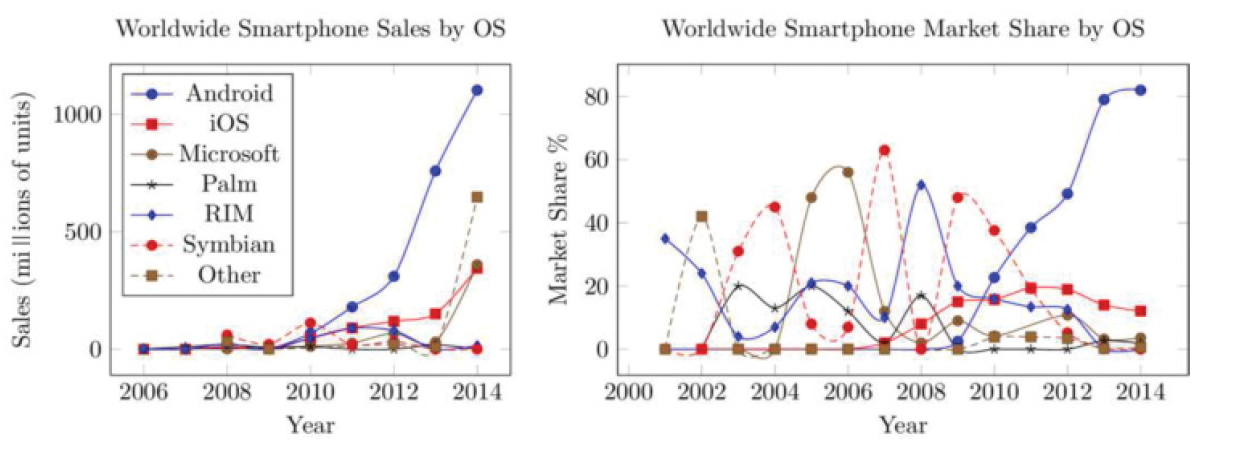
\includegraphics[scale=0.45]{smartphonemarketshare.PNG}}
        \label{lbl_smartphone_market_share}
        \caption{Smartphone market share, ~\cite[fig 1]{Tam:2017:EAM:3022634.3017427}}
\end{figure}
\begin{figure}[h!]
        \centerline{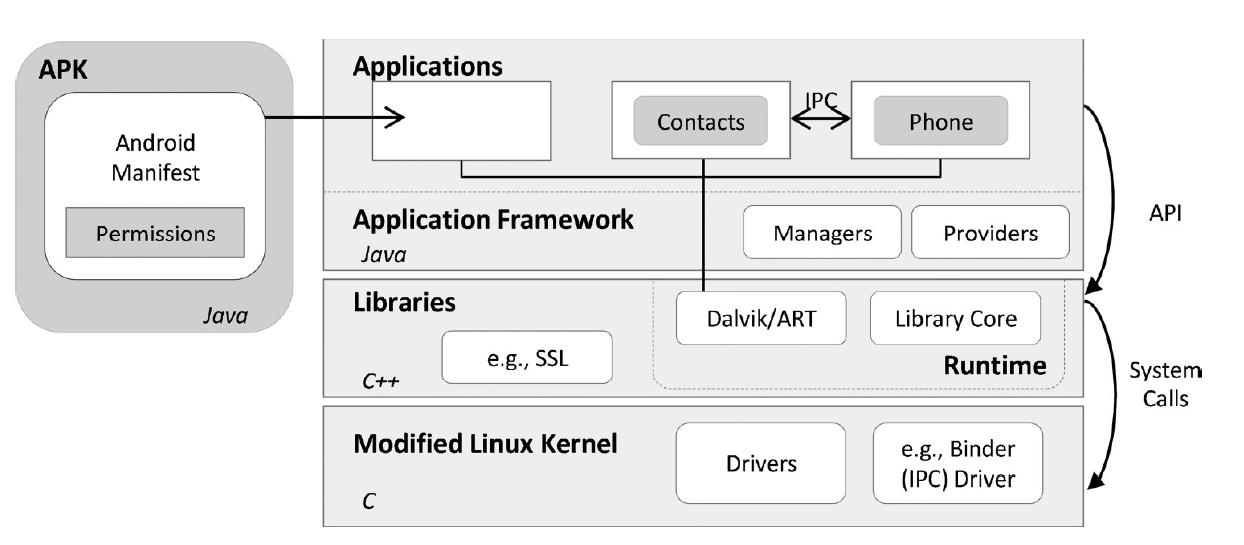
\includegraphics[scale=0.45]{androidlinuxkernel.PNG}}
        \caption{Overview of Android Operating System Architecture ~\cite[fig 2]{Tam:2017:EAM:3022634.3017427}}
        \label{lbl_linux_kernl}
\end{figure}
These graphs are important tools for conveying complex data to the readers. Since the authors traverse the evolution of malware proliferation in Android OS from the year 2010 to 2015, there are graphs to show progression of a single data annually, like mobile usage among people and worldwide smartphone market shares. Another good example of visual aid is the description of Android Linux kernel as shown in Figure \ref{lbl_linux_kernl}. Any reader would appreciate the clarity of the system blocks in this architectural diagram. \\
\begin{figure}[h!]
        \centerline{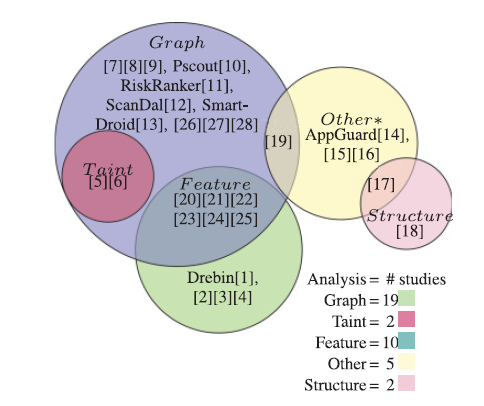
\includegraphics[scale=0.45]{venn_diagram.PNG}}
        \caption{Venn diagram of static analysis methods ~\cite[fig 3 b]{Tam:2017:EAM:3022634.3017427}}
        \label{lbl_venn}
\end{figure}
In Figure ~\ref{lbl_venn}, the authors' citations overwhelm the Venn diagram. The Venn diagram tries to explain the different static analysis methods used in Android OS. The authors could have removed the citations to a separate table to make the figure cleaner. This Venn diagram should have had only the static analysis methods and descriptions. Thus, in this particular case, the authors' purpose of using the Venn diagram is defeated.\\

\section*{Readability of the Article}
        The readability of this article is analyzed and assessed using the sections \enquote{Characteristics of a Technical Document} and \enquote{Measures of Excellence in Technical Documents} from ~\cite{markel_selber_2019_intro}.

\subsection*{\textit{Characteristics of Technical Writing}}
%Working collaboratively the authors, using the partition organization method and a visual aid, help their readers solve problems by describing how the human members of human-machine groups can learn from the 7 virtues. They reflect their organizations goals and culture by continuing to work toward better understanding human and machine cognition.
        The five authors of this article have worked collaboratively using the methods of \textit{classification}, \textit{comparison and contrast}, and \textit{problems-methods-solution} ~\cite{markel_selber_2018_org_info} to organize the information in this technical paper. The authors use \textit{cause and effect} pattern as described in ~\cite{markel_selber_2018_org_info} to depict the \enquote{time vs mobile OS usage} and \enquote{time vs malware proliferation} graphs. Statistical information used by the authors demonstrate that they have been able to monitor the best information in the area for Android OS and malware analysis.

\subsection*{\textit{Measures of Excellence in Technical Writing}}
%The authors are being honest when they depict failures in the DRC. Using the failures to describe what problems the 7 virtues could help solve increases the comprehensiveness of the article. The partition method of information organization aided in the clarity of the article. The authors also make the article more accessible by refraining from data heavy wording and instead included descriptions of events to describe the robot’s performance during the DRC.
% check for honest, clarity, accuracy, comprehensiveness, usability, conciseness, professional appearance, corectness.
The authors' research has been thorough. They have been \textit{honest} in their approach to the problem by citing statistical data. The usage of diagrams to explain architecture brings out \textit{clarity}. \textit{Accuracy, comprehensiveness and conciseness} have been the key focus for the authors and they are consistent with the \textit{problems-methods-solution} ~\cite{markel_selber_2018_org_info} approach in the paper. The document is written following the APA style, which provides a \textit{professional appearance} to the document. The document is \textit{usable} for future studies because of the data that the authors use to substantiate their arguments on malware solutions. In terms of \textit{correctness}, the authors have reviewed the document well as there are hardly any linguistic errors.


\section*{Scientific Validity of the Article}
%The article is written as an essay describing the authors’ findings after the event. The model used is to connect issues found during the DRC to a virtue and then to explain the lessons learned.
The authors of this paper describe Android architecture with a few diagrams. This is important for the reader who may not be familiar with the Android architecture. It must be noted here that though Android OS has a Linux kernel, the application architecture is different. This is because most of the mobile devices that have Android OS use the ARM hardware architecture, smaller power requirements, different storage hardware, etc.\\ 
        The usage of tables to illustrate different multi variable comparison is very apt. This helps to read the document more effectively and identify the points of differentiation with greater clarity. The authors use graphs to demonstrate single variable changes over the years, for example, Fig 1~\cite{Tam:2017:EAM:3022634.3017427}. The explanations of the dynamic analysis and static analysis are written with great detail. Other mobile operating systems are detailed in this paper. I think this is redundant because the focus of the paper is on Android OS malware. It was unnecessary to explain any of the other mobile operating systems as the security features of those devices are not in the scope of this research. In this paper, the authors should have provided details on Virtual Machine (VM) and Just In Time (JIT) compilation, as there are variants of implementations. VM and JIT are integral parts to devise any security mechanism in Android OS.

\subsection*{\textit{Scientific method:}}
%The author’s scientific method consisted of asking the question, how can we solve human-machine teamwork issues using 7 virtues? Then using the DRC to perform field research it was determined how the 7 virtues improved human-machine teamwork. Lastly conclusions were drawn by illustrating lessons from the DRC that enabled connections to the 7 virtues. 
The authors have researched extensively over 100 technical papers. To substantiate their argument, the authors have compared papers and their approaches on malware detection. This technical paper is full of references of statistics like, growth percentage of malware year over year, usage of different mobile operating systems, financial incentives of a malware, etc. The authors also look at the types of static analysis methods and dynamic analysis methods. It looks into different techniques of dynamic analysis. In this paper, the authors conclude with empirical evidence that a hybrid approach would be the way for the future of malware analysis and detection. The finding of the researchers are significant because the authors realize that mobile device ecosystem is dynamic and only a hybrid approach will lead to an effective solution for malware detection.
In the Taxonomy of Mobile Malware Analysis ~\cite{Tam:2017:EAM:3022634.3017427} section of the technical paper, the authors detail the ineffectiveness of malware detection, using binary signature analysis. The malware could evade detection by rearranging the text or the data section of malware binary. This creates a challenge and opportunity to the researchers to look for newer techniques of malware detection. The authors look into different techniques used in static code analysis, dynamic code analysis and hybrid approach at length.\\
To explain the dynamic analysis method, the authors research into the Application Programming Interface (API) and its interaction with the kernel, to build up the security hole context. Since dynamic analysis can expose the executable part of the source code (for malware analysis), the authors describe different input techniques that could be used to create a graph to explore the different paths of code execution. Dynamic analysis needs to be done at different architectural layers (application, kernel, device drivers, hardware interactions, etc.).\\
The authors also look into the evolution of the evasion techniques used by the malware. One of the simple techniques that the malware uses is to run the application at odd hours when the users are not using the devices. The authors identify that permission infrastructure is the weak point in the Android architecture. In this paper, the authors try to pivot on this architectural issue and try to devise different malware analysis and detection methods.

\subsection*{\textit{Proposed Solutions}}\label{ref:paper_sol}
The number of different mobile devices that are available complicates the problem of malware detection. It's hard to perform the analysis of the malware in all the target (available) mobile devices. The authors \textit{propose} a hybrid approach that combines static and dynamic analysis methods with use of VM to simulate the multitude of target android devices for malware detection. The VM can be simulated to operate like a real hardware with certain changes in the software. \\
In this paper, the authors detail another hybrid approach in which static and dynamic analysis methods along with machine learning (ML) could be used for analysis of the malware. This method seems to be superior because it can scale to support the huge number of different hardware Android OS. \\ 
As alternative approaches, the authors explore other techniques of identifying malware like, using network traffic analysis, code coverage of API interfaces, monitoring system calls, creation of application dependency graphs for all the applications running, information-flow among the application and operating system infrastructure, inter-process communication analysis, hardware analysis, and application metadata analysis. The authors also mention that detection of malware after malware analysis is a \textit{classification} problem. In situations where malware cannot be identified using binary classification, different attributes of the malware need to be analyzed, thereby translating the analysis problem to a multiple class \textit{stochastic} problem. \\ 
\subsection*{\textit{Scope of Future Work}}\label{ref:paper_scope}
The authors state that the future of the Android malware research is in pursuing the path of hybrid approach that uses static analysis, dynamic analysis, and ML along with the use of virtual machines to simulate target hardware. The advances in parallel computing would allow future researchers to follow the hybrid approach of malware analysis. The authors highlight the advantages of performing code coverage analysis on the applications using the hybrid mechanism. Code coverage method can present different branches of execution, which would help in identifying the weak links in an application. Since malware has started evading detection in virtualised environment, one area of research would be to use virtualization to detect malware.

\subsection*{\textit{Unanswered Questions}}\label{ref:critique_method}
One of the primary reasons for the proliferation of the Android malware is the failure of App store to check for malicious applications. In this paper, the authors should have detailed the mechanism of application upload and application distribution in App store. A section should have been written about this in the technical paper. The authors do not describe the installation process of application in Android OS. Details on the tools that had been used in this research is missing. The authors do not rule out or talk about the flaws in ARM architecture, which could be the reason for malware proliferation in Android.

\section*{Conclusion}
The authors of this technical paper mention that they studied a wide range of Android malware analysis and detection frameworks. The technical paper created the context by describing the threat-landscape for mobile devices, followed by the evaluation of different malware detection techniques and solutions. The authors think that they have discussed threats and solutions for android devices and that they have been able to provide a superior solution than those available.\\
The authors acknowledge UK EPSRC grant EP/L022710/1 and Ministry of Science, Technology and Innovation, under Grant eScienceFund 01-01-03-SF0914 for funding their research for this paper.

%The San Jose State University Cybersecurity program primarily includes courses revolving around cybersecurity, which was emphasized both implicitly and explicitly by this article.  Although there was no specific problem this survey attempted to find a solution for, the report did provide a detailed back story on why we got to where we are today and the continued and increased need of cybersecurity in the automotive industry, especially as the world races towards autonomous vehicles.  

\subsection*{\textit{Usefulness to your major}}
%The current robot revolution is ever present in the mind of the Industrial/Systems Engineer. Our field will be part of the solution to the issues that arise when autonomous robots become commonplace in industry. Facilities will need to be designed in ways that the robots can navigate without error, employees will need to be trained in human-machine interaction and how to best work together, and the psychological impact of having to depend on an autonomous partner are some ways this subject is of use to the Industrial/Systems Engineer major.
The San Jose State University graduate program in software engineering focuses on cybersecurity. Mobile security is a relevant topic in cybersecurity. In this technical article, the evolution of malware in Android OS is highlighted and a solution to mitigate the proliferation of malware is proposed. Reading this technical paper made me aware of the hybrid method of malware elimination in Android OS.

%\subsection*{\textit{Recommendations about improvements for clarity}}
%Although the article’s information was highly accessible it would have benefited from a better description of the scientific method and/or design method used. The article lists results of the DRC, lessons learned from the results, and the virtue that fits best. This model is easily read but still lacks the technical bent required by the journal’s audience.

%\bibliographystyle{apacite}
\bibliographystyle{apalike}
\bibliography{memo-reportAnalysisOfAProfessionalJournalArticle}

\end{document}
